\documentclass{article}

\usepackage[margin=1in]{geometry}
\usepackage{fancyvrb, fancyhdr, inconsolata, amsmath}
\usepackage{graphicx}

\usepackage{enumitem}

\author{Long Nguyen; Collaborator: Joseph Lin}
\title{6.814 - Problem Set 2}

\begin{document}

\maketitle

\small

\section*{Part I - Query Plans \& Cost Models}

\begin{enumerate}

\item Using the command \verb|\d movies|, I retrieved the following indexes for \verb|movies|.

\begin{Verbatim}
Indexes:
"movies_pkey" PRIMARY KEY, btree (id)
"movies_title" btree (title)
\end{Verbatim}

\item Postgres chooses the following sequential scan query for \verb|select title from movies|.

\begin{Verbatim}
QUERY PLAN
---------------------------------------------------------------
Seq Scan on movies  (cost=0.00..8418.65 rows=464065 width=18)
(1 row)
\end{Verbatim}

This plan is not any different from the plan on the previous page, but given the \verb|btree| index defined on \verb|movies|, we could have chosen another possible query plan, one based on the B-tree.

\item I ran \verb|explain select title from movies order by title;| and got the following output.

\begin{Verbatim}
QUERY PLAN
------------------------------------------------------------------------------------------
Index Only Scan using movies_title on movies  (cost=0.42..15677.40 rows=464065 width=18)
(1 row)
\end{Verbatim}

The previous plan retrieves all movie titles sequentially, but the plan in this query must retrieve movies in order, so it accesses \emph{only} on the B-tree index to get sorted titles.

\item The command \texttt{explain select title, year from movies order by
title} yielded the following output.

\begin{Verbatim}
QUERY PLAN
-------------------------------------------------------------------------------------
Index Scan using movies_title on movies  (cost=0.42..30786.82 rows=464065 width=22)
(1 row)
\end{Verbatim}

In this query, we don't have an index-\emph{only} scan. This is because while we are still sorting by \verb|title|, we need to also retrieve \verb|year| from the heap. The previous question made use of a scan that would only refer to the B-tree, conveniently because \verb|title| was the only criterion we had for selection.

\item Because \verb|people_reduced| does not have the extra column with type \verb|character(20000)|, a sequential scan is the best option, as there is no I/O overhead in reading so much more data, and sequentially scanning only 1000 rows is going to be more efficient than using the index (random access overhead).

On the other hand, \verb|people_wide| has the extra column, so performing a sequential scan, while sensible to get all the names without sorting, makes little sense if I/O operations are going to be wasted on the extra field, especially if each can be up to 20000 characters long. Thus, using only the B-tree index to scan for the names is going to be cheaper in this case.

% 6
\item First, I ran sequential and index-only scans on the query for \verb|people_reduced|. Their outputs are below.
\begin{verbatim}
QUERY PLAN                                                   
-----------------------------------------------------------------
Seq Scan on people_reduced  (cost=0.00..18.00 rows=1000 width=14) 
(actual time=0.050..0.271 rows=1000 loops=1)
Planning time: 0.029 ms
Execution time: 0.338 ms

QUERY PLAN                                                                    
-----------------------------------------------------------------
Index Only Scan using people_reduced_name on people_reduced  (cost=0.28..43.27 rows=1000 width=14) 
(actual time=0.099..0.294 rows=1000 loops=1)
Heap Fetches: 0
Planning time: 0.060 ms
Execution time: 0.369 ms
\end{verbatim}
As we see, indeed, the sequential scan on \verb|people_reduced| was the right plan, and the query optimizer was correct. Now, I run sequential and index-only scans on the query for \verb|people_wide|.
\begin{verbatim}
QUERY PLAN                                                  
-----------------------------------------------------------------
Seq Scan on people_wide  (cost=0.00..50.00 rows=1000 width=14) 
(actual time=0.043..0.562 rows=1000 loops=1)
Planning time: 0.024 ms
Execution time: 0.630 ms

QUERY PLAN                                                                 
-----------------------------------------------------------------
Index Only Scan using people_wide_name on people_wide  (cost=0.28..43.27 rows=1000 width=14) 
(actual time=0.087..0.260 rows=1000 loops=1)
Heap Fetches: 0
Planning time: 0.037 ms
Execution time: 0.326 ms
\end{verbatim}
We see that the query optimizer was right again, and by more than its estimated costs. There is only a $50-43.27$ difference in estimated cost, but the runtime of a sequential scan on \verb|people_wide| is almost double that of an index-only scan.

% 7
\item We have to keep in mind that Postgres's query planner/optimizer isn't a perfect proxy for how our query will actually run. The optimizer makes certain assumptions about the hardware (in this case, the Athena cluster) and the row estimates are only based off of selectivity functions run on the samples chosen. Thus, the huge discrepancy between the estimated costs of the two queries is large and valid, and they don't necessarily correlate completely to actual query execution. 

As for the actual costs, it makes sense when considering how many predicate operations we have to perform respectively for each one. We have to filter out 45 rows for the second query, whereas we only have to filter out 10 for the first. Flushing these out to the user is also dependent on how many results we got.

Verbatim from the \verb|EXPLAIN| documentation provided in the link given in the problem set document: ``In particular, the cost does not consider the time spent transmitting result rows to the client, which could be an important factor in the real elapsed time.''

% 8
\item Below are the full diagrams for both Q2005 and Q2050.

\begin{center}

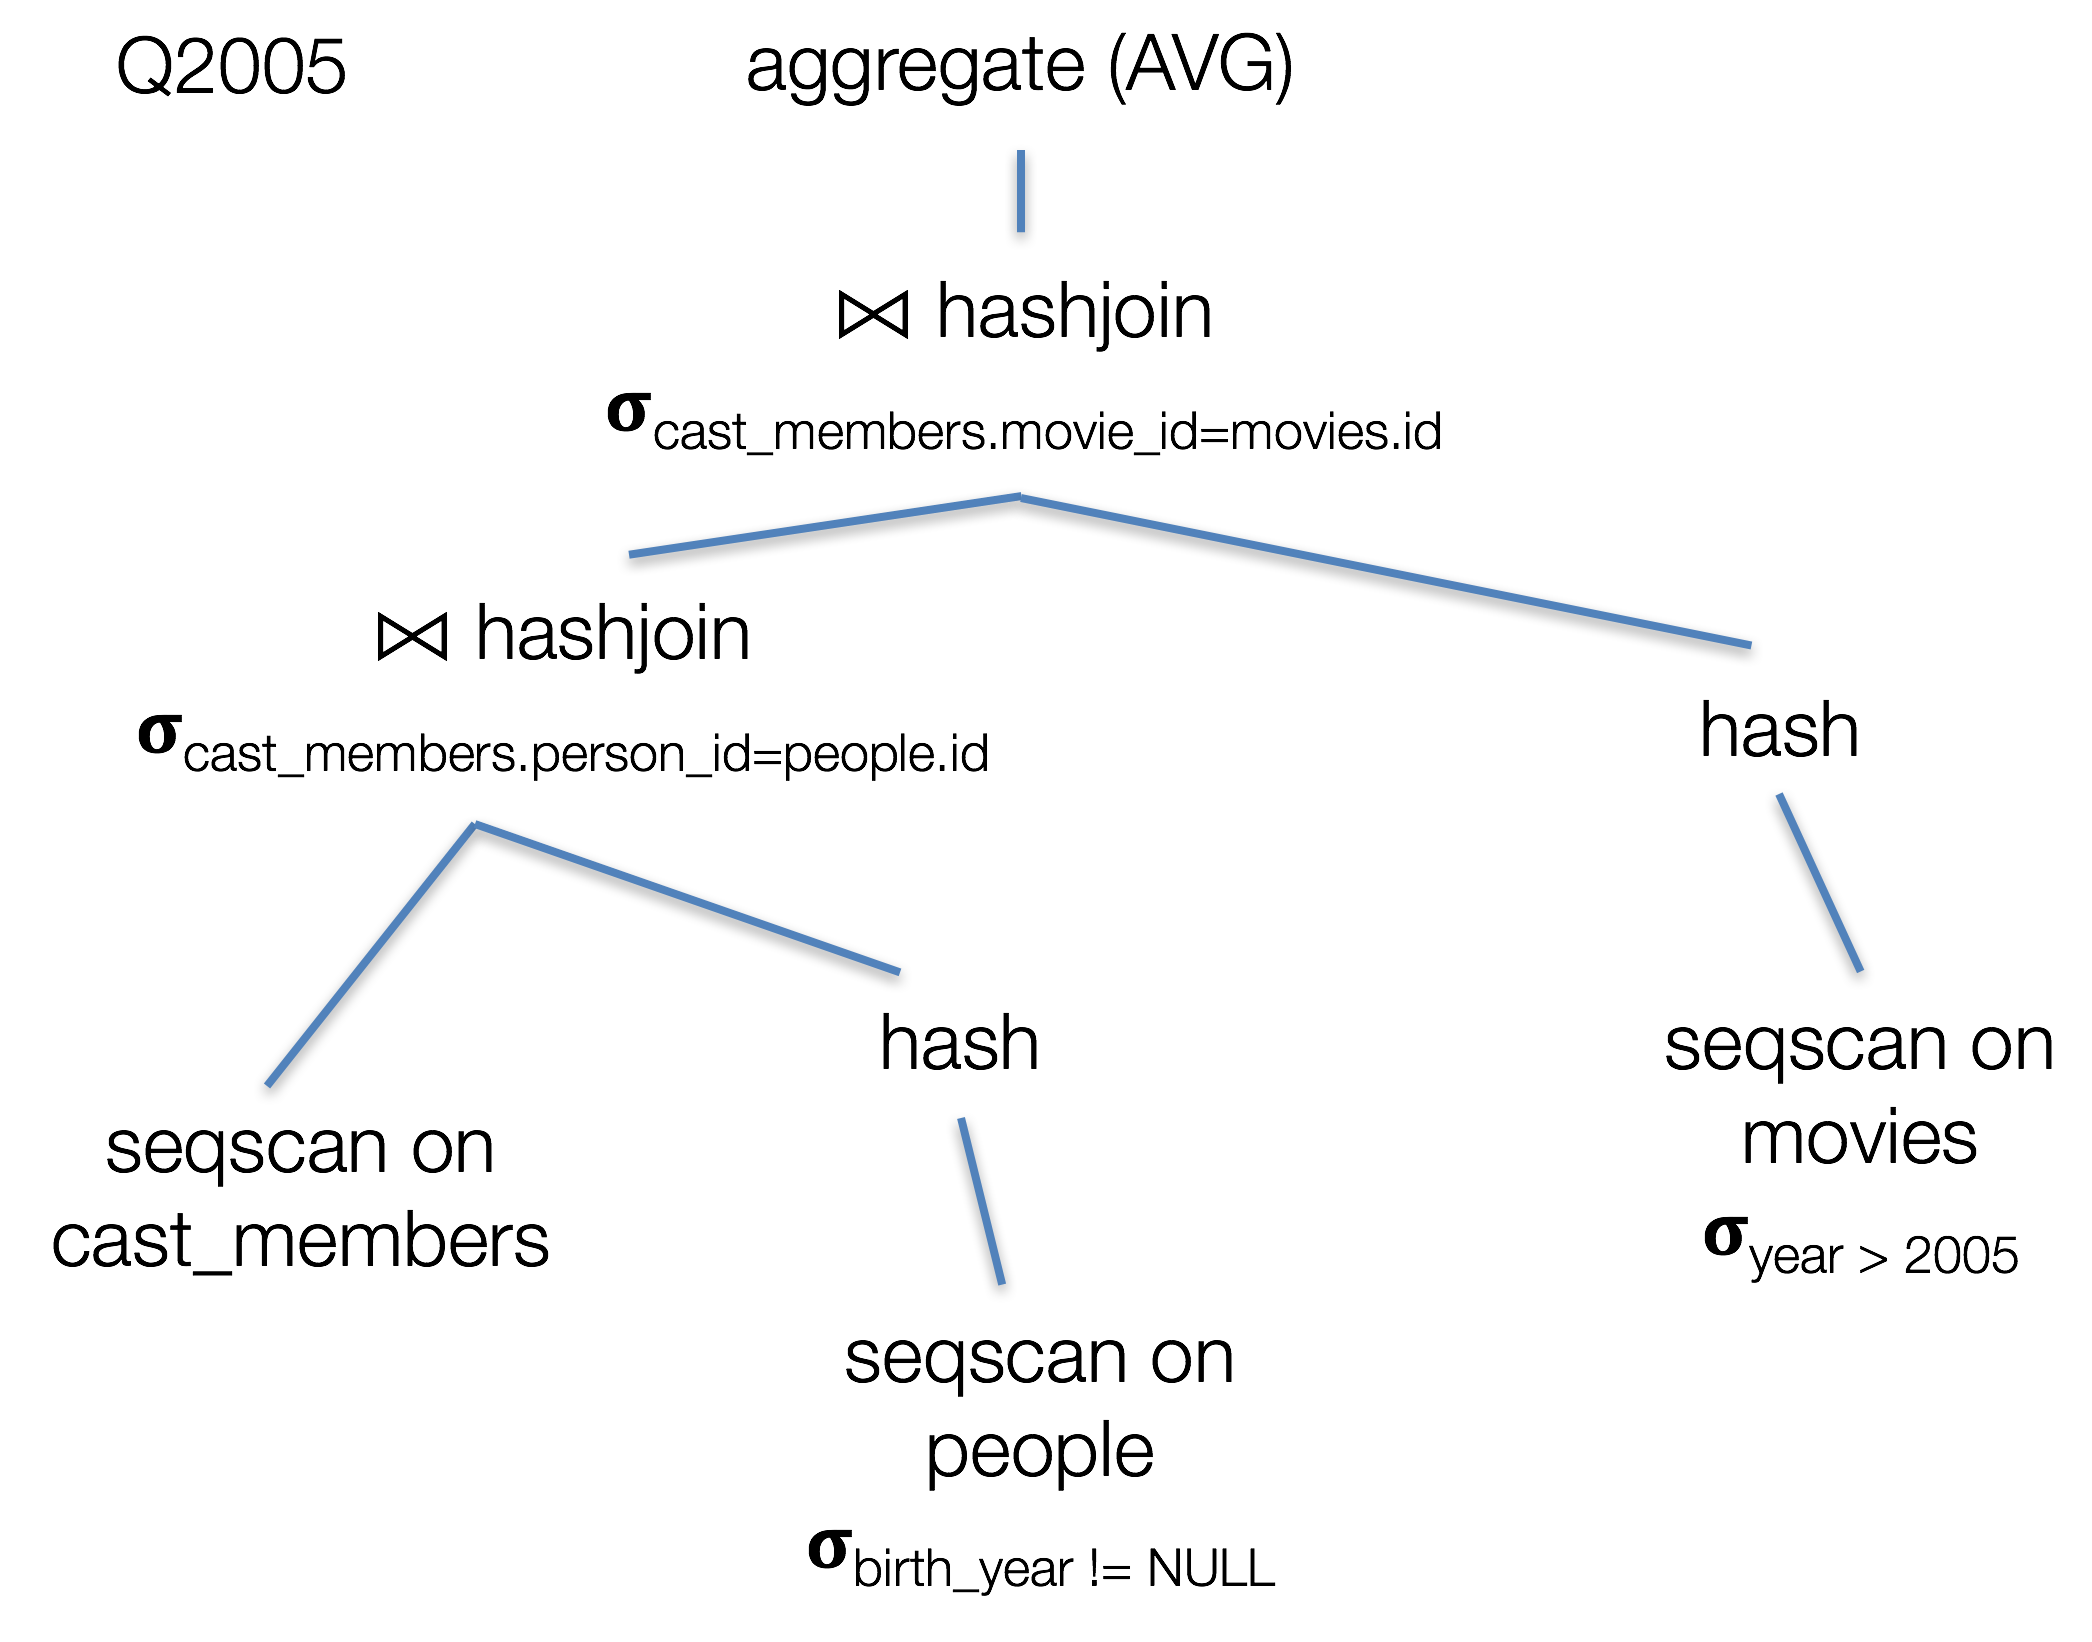
\includegraphics[scale=0.3]{q2005.png}

\vspace{20px}

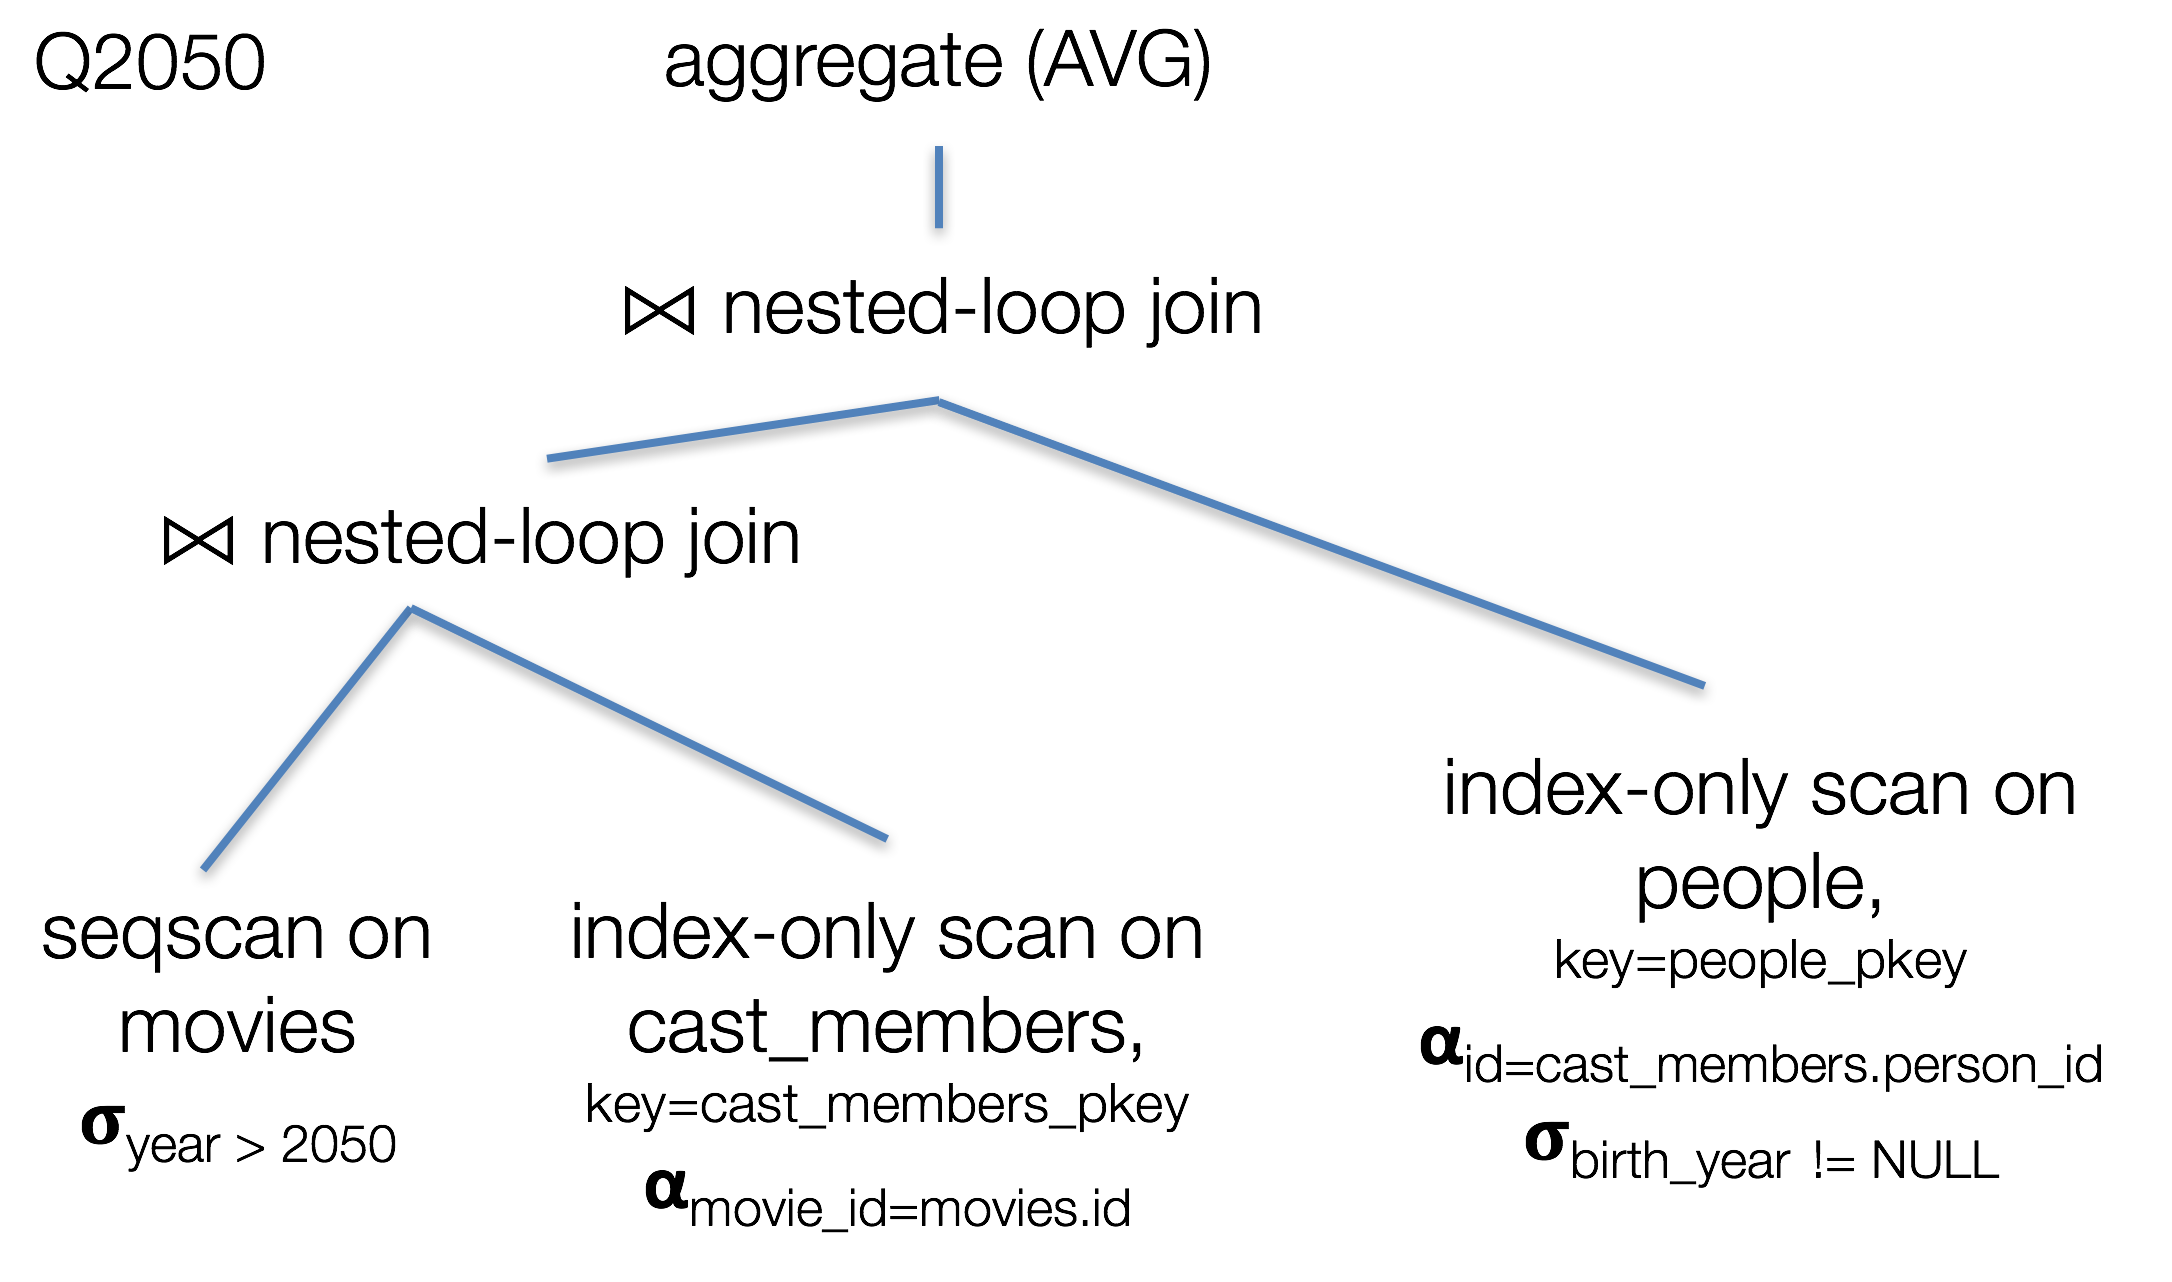
\includegraphics[scale=0.3]{q2050.png}

\end{center}

\vspace{20px}

% 9
\item Refer to 8.

% 10
\item Refer to 8.

% 11
\item On the hashjoin between \verb|cast_members| and \verb|people| in Q2005, I notice that PSQL expected 548809 result rows from the join, but the actual amount turned out to be 1391484, more than double that.

Also, on all the scans and nested-loop joins in Q2050, I notice that PSQL overshot its estimates of output cardinality by way more than factors of 2. For example, the nested-loop join between \verb|movies| and \verb|cast_members| produced \emph{only 6 rows} when PSQL predicted 165.

% 12
\item The query planner changes from hash joins to nested-loop joins starting at the year 2018. This is the only point at which it changes plans. It does so because our filter becomes increasingly selective. When querying at the very beginning, \verb|WHERE year > 1893|, we are looking over the \emph{entire dataset}, so hashing and then joining is much more efficient than using nested loops.

More quantitatively, let us consider how the selectivity changes. We use \verb|...| for brevity.

Consider the filter \verb|WHERE year > 1893|, where we expect to have 508297 output rows, the \emph{entire dataset}.
\begin{verbatim}
                                       QUERY PLAN                                        
-----------------------------------------------------------------------------------------
 Aggregate  (cost=141886.36..141886.37 rows=1 width=4)
   ->  Hash Join  (cost=35967.04..140615.62 rows=508297 width=4)
         Hash Cond: (cast_members.movie_id = movies.id)
         ->  Hash Join  (cost=21015.61..114407.12 rows=548809 width=14)
               Hash Cond: (cast_members.person_id = people.id)
               ->  Seq Scan on cast_members  (cost=0.00..54568.21 rows=3333521 width=20)
         ...
\end{verbatim}

Now consider 1955, between 2018 and 1893. We still have 418333 rows of expected output, so the hash join is still valid.
\begin{verbatim}
                                       QUERY PLAN                                        
-----------------------------------------------------------------------------------------
 Aggregate  (cost=138438.88..138438.89 rows=1 width=4)
   ->  Hash Join  (cost=35016.12..137393.04 rows=418333 width=4)
         Hash Cond: (cast_members.movie_id = movies.id)
         ->  Hash Join  (cost=21015.61..114407.12 rows=548809 width=14)
               Hash Cond: (cast_members.person_id = people.id)
               ->  Seq Scan on cast_members  (cost=0.00..54568.21 rows=3333521 width=20)
               ->  Hash  (cost=18744.75..18744.75 rows=181669 width=14)
         ...
\end{verbatim}

Now, the breakpoint. 2017 expects 7955 output rows.
\begin{verbatim}
                                       QUERY PLAN
-----------------------------------------------------------------------------------------
 Aggregate  (cost=58245.99..58246.00 rows=1 width=4)
   ->  Hash Join  (cost=21016.04..58226.10 rows=7955 width=4)
         Hash Cond: (cast_members.person_id = people.id)
         ->  Nested Loop  (cost=0.43..36647.71 rows=48322 width=10)
            ...
\end{verbatim}

Now transition to 2018, where the expected output cardinality has decreased \emph{significantly} to 496.
\begin{verbatim}
                                       QUERY PLAN
-----------------------------------------------------------------------------------------
 Aggregate  (cost=12949.63..12949.64 rows=1 width=4)
   ->  Nested Loop  (cost=0.86..12948.39 rows=496 width=4)
         ->  Nested Loop  (cost=0.43..11528.11 rows=3010 width=10)
               ->  Seq Scan on movies  (cost=0.00..9578.81 rows=419 width=10)
                     Filter: (year > 2018)
         ...
\end{verbatim}

At this point, is it really worth it to hash and then join anymore, when we have such little expected cardinality? It's better now to brute-force our way through with nested-loop joins, which may even prove more efficient than the former.

Let's see if the query planner is actually switching correctly. We run \verb|EXPLAIN ANALYZE| on this switch point.

\footnotesize
\begin{verbatim}
> 2017
 Aggregate  (cost=58245.99..58246.00 rows=1 width=4) (actual time=423.223..423.223 rows=1 loops=1)
   ->  Hash Join  (cost=21016.04..58226.10 rows=7955 width=4) (actual time=199.922..421.803 rows=9251 loops=1)
         Hash Cond: (cast_members.person_id = people.id)

> 2018
 Aggregate  (cost=12949.63..12949.64 rows=1 width=4) (actual time=127.325..127.325 rows=1 loops=1)
   ->  Nested Loop  (cost=0.86..12948.39 rows=496 width=4) (actual time=26.743..127.086 rows=851 loops=1)
\end{verbatim}
\small

Indeed, the actual output cardinality decreases significantly by more than a factor of 10 within just this one transition. The query planner was right in switching to nested loops.

\end{enumerate}

\section*{Part II - Query Plans \& Access Methods}

\begin{enumerate}[resume]
	
	% 13
	\item If we have no indexes, then using a nested-loop join on \verb|customer| and \verb|orders| will benefit us greatly, since the inner table \verb|customer| is only of cardinality $SF\cdot150,000$. Then, once we've done this join, we'll use the grace hash join between it and \verb|lineitem|, which is far too large to fit into memory.

	The image of my proposed query plan is below.

	\begin{center}
	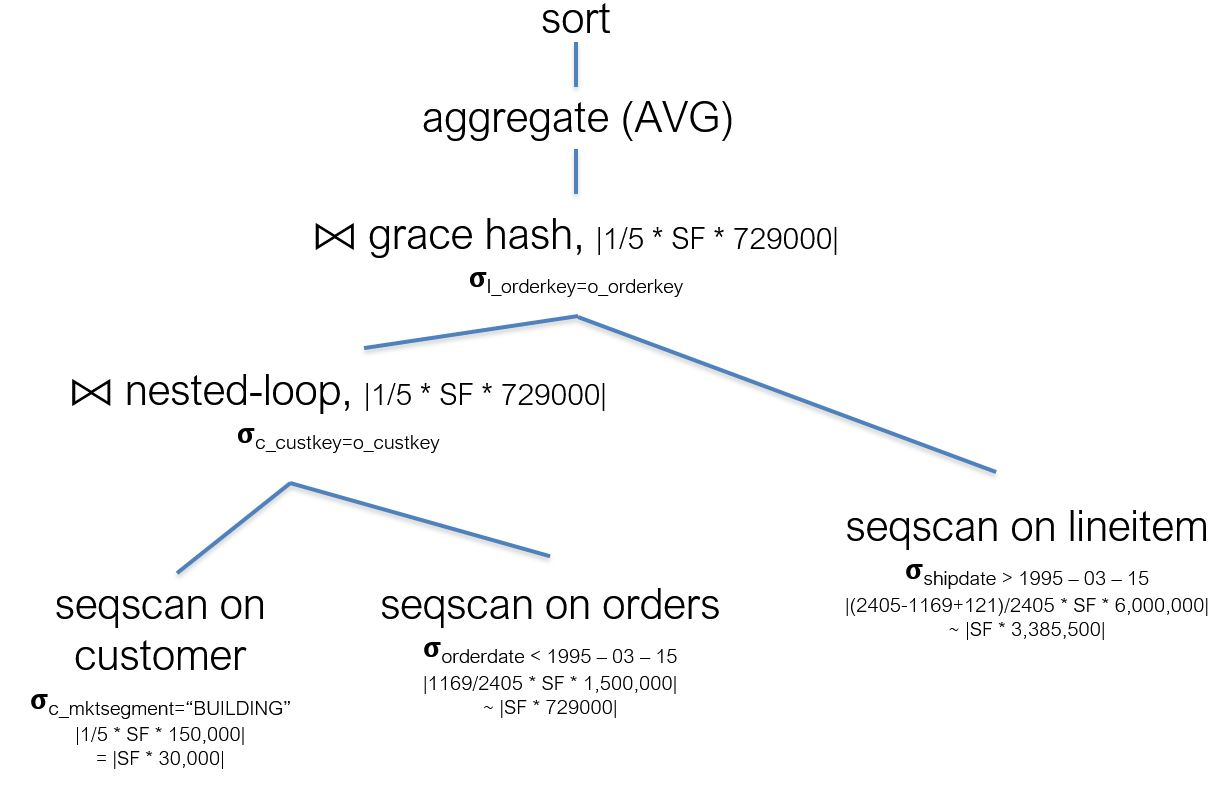
\includegraphics[scale=0.5]{q13.JPG}
	\end{center}

	Assuming uniform distributions, we should expect to have 1/5th of \verb|customer| filtered from our scan with all the market segments. Likewise, there are 1169 days from the beginning of the range until March 15, 1995 (out of 2405 possible days in the range), and calculations were made accordingly. Then, we assume again uniformity in the sense that 1/5th of \verb|orders| belongs to the 1/5th customers we filtered out for. Thus, we are bounded by $1/5\cdot SF\cdot 729000$. 

	A note: \emph{a nested-loop join could've worked for the final join, because our expected output is only 412Mb and can still fit into memory, but only if our uniform distribution assumption actually holds in practice. For generality, I chose the grace hash join instead.}

	% 14
	\item For this query plan, we first sequentially scan \verb|customer|, so that's 268.5Mb. Then, we put \verb|customer| in our 1Gb memory to make our nested-loop join quicker. Now, we read \verb|orders| (with the predicate filtering too) for the nested-loop join, and this is 1560Mb. Finally, we perform grace hash on our intermediate join result (412Mb) and \verb|lineitem| (6720Mb), so we must scan \verb|lineitem| and our previous output of the nested-loop join (formulas as taken from lecture slides).

	Altogether, this is \begin{equation*}
	\frac{268.5+1560+3(412+6720)}{100}=232 \text{ seconds = 3.9 minutes}.
	\end{equation*}

	% 15
	\item Now that we are only concerned with efficiency and don't care about insert time, we can use clustered indexes to save ourselves the need of sequentially scanning each table in its entirety. We cluster each heap file based on the useful rangescan that we need to perform: thus, cluster \verb|lineitem| by \verb|shipdate|, \verb|customer| by \verb|mktsegment|, and \verb|orders| by \verb|orderdate|. This gets rid of the entire overhead that we have in needing to scan each entire table during our joins, and now, we only need to do a disk seek and then read sequentially all this data that meets our criteria. This will help with efficiency.

	% 16
	\item For this query, I chose not to modify anything related to the join algorithms. We now have the choice of using index-based nested-loop joins, but I felt that sticking with the initial nested-loop join was the better option, since we're still just reading a small amount of data and either would probably work. As for the grace hash join, we still have $>3,000,000$ results expected from the scan on \verb|lineitem|, so it's probably best to just stick to the old plan where it may not fit into memory.

	The picture for this query is located below.

	\begin{center}
	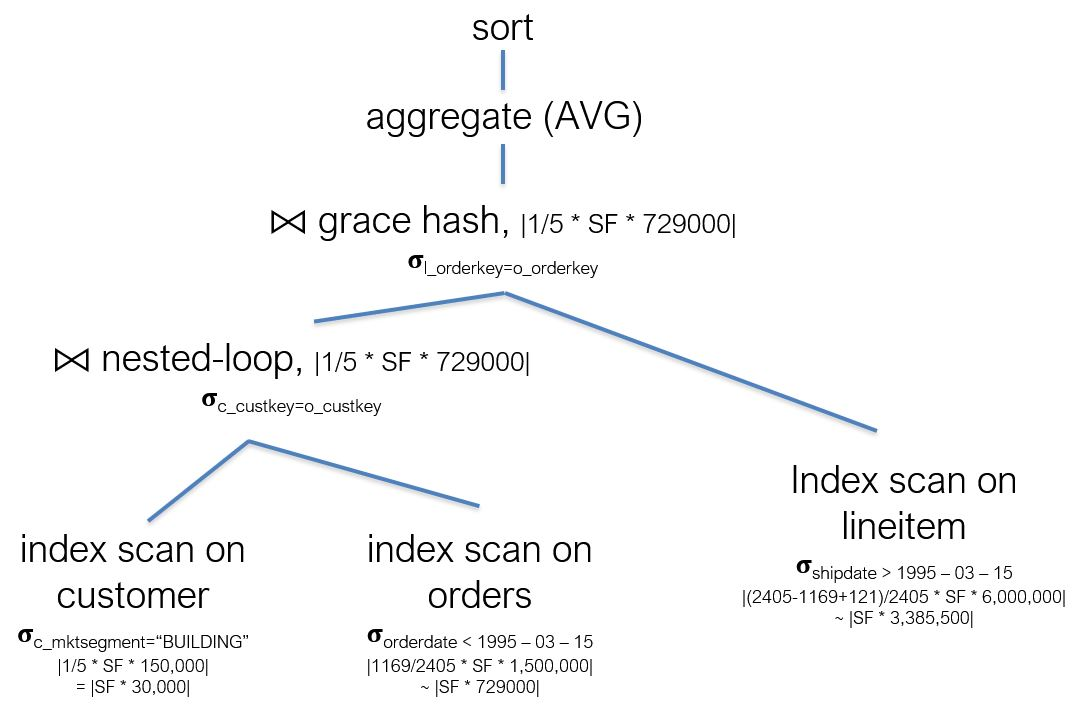
\includegraphics[scale=0.5]{q16.JPG}
	\end{center}

	% 17
	\item With our newly generated indexes, we don't have to scan the entire table sequentially to filter out what we want. Instead we can simply do a rangescan on all three tables with our B+ tree indexes. We look only at the \verb|mktsegment='BUILDING'| part of \verb|customer|, and so on regarding dates for the other two tables. Thus, our runtime is around \begin{equation*}
	\frac{\frac{1}{5}\cdot268.5+\frac{1169}{2405}\cdot1560+3(412+\frac{1357}{2405}\cdot6720)}{100}=134 \text{ seconds = 2.2 minutes.}
	\end{equation*}

\end{enumerate}

\section*{Part III - Schema Design and Query Execution}

\begin{enumerate}[resume]
	
	% 18
	\item We make some assumptions. Assume that \verb|roomname| is unique, that each \verb|(firstname, lastname)| key is unique, that room pairs are connected by at most one corridor (it would be weird if a room had a backdoor that led to another corridor, etc.), and that relationships between pairs of people can only be one type (philosophically, you can be friends and enemies with a person, but practically, we assume you may only be one). Also, corridors are unique in that they have unique identifiers (like name, or ID, etc.).

	Now, we consider functional dependencies.

	\begin{itemize}
		\item room $\rightarrow$ room size
		\item (first, last) $\rightarrow$ birthday
		\item relationship/pair $\rightarrow$ type of relationship
	\end{itemize}

	% 19
	\item Consider the ER diagram below.

	\begin{center}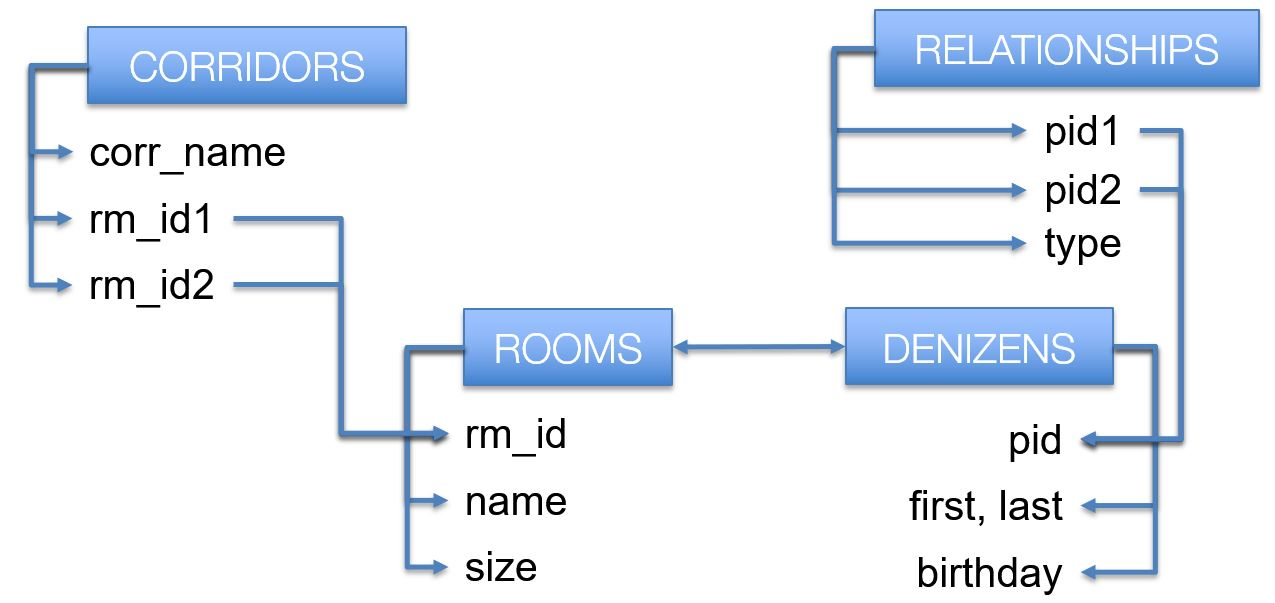
\includegraphics[scale=0.35]{er_diagram.JPG}\end{center}

	I drew it this way for a few reasons:
	\begin{itemize}
		\item Double-sided arrow between DENIZENS and ROOMS because the problem mentions that rooms may have 0 or more, and denizens may reside in 0 or more.
		\item Relationships consist of two people, which directly relate to the DENIZENS people.
		\item Corridors uniquely connect two rooms together, and this relates to the ROOMS table.
	\end{itemize}

	% 20
	\item Following the ER diagram drawn previously, my BCNF schema is as follows: \verb|rooms(rid, rname, rsize)|, \verb|corridors(cname, rmid1, rmid2)|, \verb|denizens(pid, first, last, bday)|, \verb|relationships(pid1, pid2, type)|, and \verb|residents(rid, pid)|.

	For \verb|rooms|, primary key is \verb|rid|, secondary key is \verb|rname|.

	For \verb|corridors|, primary key is \verb|cname|.

	For \verb|denizens|, primary key is \verb|pid|, secondary key is \verb|(first, last)|.

	For \verb|relationships|, primary key is \verb|(pid1, pid2)|.

    For \verb|residents|, the primary key is \verb|(rid, pid)|.

	% 21
    \item My schema is indeed redundancy and anomaly-free. For every FD mentioned previously, the left side is a key of its respective table. Also, by introducing the \verb|residents| table, we capture the many-to-many relationship between \verb|denizens| and \verb|rooms| without being vulnerable to update anomalies. We can delete denizens and rooms from their respective tables while still maintaining accurate information regarding corridors and relationships between denizens.

    % 22
    \item If we wanted to ensure that each denizen has more friends (or be evicted otherwise), we can do a check on insertion. For example, we could query to check for the amount of friends and enemies a person has (easy queries on the \verb|relationships| table), and if it's satisfied, insert. The constraint is thus enforced by construction, and proof by induction on the $i$th insertion is left beyond the scope of this problem.

    % 23 
    \item If each denizen should live in exactly one room, then it's simple: we drop the \verb|residents| table, and we add a new field \verb|livingroom| field to the \verb|denizens| table schema. Now, every denizen has a room associated with them.

    A view for this with backwards compatibility would be to generate the new table \verb|denizens'| as part of the view, where the \verb|livingroom| field is just one chosen arbitrarily from however many rooms a denizen lived in under the old schema.

    This works, but it obviously can't handle when we want to specify exactly what room the denizen could have lived in out of $x$ rooms the denizen lived in under the old schema. \verb|denizens'| can only take one of these.

\end{enumerate}

\end{document}
